%!TEX root = htm.tex
\subsection{Progressive HyTM with linear}
\label{sec:hytm1}
%
\begin{algorithm}[!ht]
\caption{Progressive fast-path and slow-path opaque HyTM implementation; code for transaction $T_k$}
\label{alg:inswrite}
\begin{algorithmic}[1]
  	\begin{multicols}{2}
  	{
  	\footnotesize
	\Part{Shared objects}{
		\State $v_j$, value of each t-object $X_j$ 
		\State $r_{j}$, a versioned lock for each t-object $X_j$
	}\EndPart	
	\Statex
	\Part{Process local objects}{
		\State $\Rset(T_k)$, storing $\{X_j,r_j\}$
		\State $\Wset(T_k)$, storing $\{X_j, v_j\}$
	}\EndPart
	\Statex
	\textbf{Code for fast-path transactions}
	\Statex
	\Part{$\textit{read}_k(X_j)$}\quad\Comment{fast-path}{
		\State $\textit{ov}_j := \Read(v_j)$ \Comment{cached read} \label{line:lin1}
		\State $\textit{or}_j := \Read(r_j)$ \Comment{uncached read}
		\If{$\textit{or}_j$ $\mathrel{\&}1$}  \label{line:hread}
			\Return $A_k$ \EndReturn
		\EndIf
		
		\Return $\textit{ov}_j$ \EndReturn
		
   	 }\EndPart
	\Statex
	%\Comment{What is the best strategy to buffer writes?}
	\Part{$\textit{write}_k(X_j,v)$}{\quad\Comment{fast-path}
		\State $\textit{or}_j := \Read(r_j)$ \Comment{cached read}
		\If{$\textit{or}_j$ $\mathrel{\&} 1$}  		
			\Return $A_k$ \EndReturn
		\EndIf
		
		\State $\Write(r_j,\textit{or}_j+2)$ \Comment{uncached write}
		\State $\Write(v_j,v)$ \Comment{uncached write} 
		\Return $\ok$ \EndReturn
		
   	}\EndPart
	\Statex
	
	\Part{$\textit{tryC}_k$()}{\quad\Comment{fast-path}
		\State $\ms{commit-cache}_i$ \label{line:lin3} \Comment{returns $C_k$ or $A_k$}
  	 }\EndPart
  	 
  	 \Statex
  	\Part{Function: $\lit{release}(Q)$}{
  		\ForAll{$X_j \in Q$}	
 			\State $r_j.\lit{write}(or_j+1)$ \label{line:rel1}	
		\EndFor
		
	}\EndPart
 	\Statex
	\Part{Function: $\lit{acquire}(Q)$}{
  		\ForAll{$X_j \in Q$}	
 			\If{ $r_j.\lit{setV}()$} \label{line:acq1}
			  \State $\ms{Lset}(T_k):=\ms{Lset}(T_k)\cup \{X_j\}$
			  \Return $\true$ \EndReturn
			\EndIf
			\State $\lit{release}(\ms{Lset}(T_k))$
			\Return $\false$ \EndReturn
		\EndFor
		
	}\EndPart
	\Statex
	\Statex \Comment{Implement using LL/SC on Power8}
	\Part{Function: $\lit{setV}()$}{
% 		\State $\ms{success} \gets \lit{false}$
% 		
% 		\While{($\neg \ms{success}$)} \Comment {spin until we get the lock}
		%\State $\ms{or}_j \gets$ $r_j.\Read()$ $\mathrel{\&}1111...1110$
		\If{$r_j$.CAS($or_j$, $or_j+1$)} 
		  \Return $\false$  \EndReturn
		\EndIf
		\Return $\true$ \EndReturn
	}\EndPart
  	 
  	 \newpage
	\textbf{Code for slow-path transactions}
	\Statex
	\Part{\Read$_k(X_j)$}\quad\Comment{slow-path}{
		  \If{$X_j\in \Wset(T_k)$}
		    \Return $\Wset(T_k).\lit{locate}(X_j)$ \EndReturn
		  \Else
		  
		  \State $\textit{or}_j := \Read(r_j)$ \label{line:readorec}
		  \State $\textit{ov}_j := \Read(v_j)$ \label{line:read2}
		  \State $\Rset(T_k) := \Rset(T_k)\cup\{X_j,or_j\}$ \label{line:rset}
		  \If{$\textit{or}_j$ $\mathrel{\&} 1$} \label{line:abort0}	
			\Return $A_k$ \EndReturn
		  \EndIf
		 
		  \If{$\neg \lit{validate}()$} \label{line:valid}
			\Return $A_k$ \EndReturn
		  \EndIf
		  \EndIf
		  \Return $\textit{ov}_j$ \EndReturn
		
   	 }\EndPart
	\Statex
	\Part{\Write$_k(X_j,v)$}\quad\Comment{slow-path}{
		
			\State $\textit{or}_j := \Read(r_j)$
			\State $\textit{nv}_j := v$
			\If{$\textit{or}_j$ $\mathrel{\&} 1$}	
			\Return $A_k$ \EndReturn
			\EndIf
			\State $\Wset(T_k) := \Wset(T_k)\cup\{X_j,\textit{nv}_j\}$
			\Return $\ok$ \EndReturn
		
   	}\EndPart
	\Statex
	
	%\Statex	
	\Part{\TryC$_k$()}\quad\Comment{slow-path}{
		\If{$\Wset(T_k)= \emptyset$}
			\Return $C_k$ \EndReturn \label{line:return}
		\EndIf
		\If{$\lit{acquire}(\Wset(T_k))$}	\label{line:acq}
		
		\If{$\neq \lit{validate}()$} \label{line:abort3}
			\State $\lit{release}( \ms{Wset}(T_k))$ 
			\Return $A_k$ \EndReturn
		\EndIf
		\ForAll{$X_j \in \Wset(T_k)$}
	 		\State  $v_j.\lit{write}(\textit{nv}_j)$ \label{line:write}
			 
	 	\EndFor	
		  
		\State $\lit{release}(\Wset(T_k))$   \label{line:rel}	
   		\Return $C_k$ \EndReturn
   		\Else
		  \Return $A_k$ \EndReturn
		  \EndIf
   	 }\EndPart		
	 
 	
	\Statex
	\Part{Function: $\lit{validate}()$}{\quad\Comment{Validate slow-path reading transactions}
		\If{$\exists X_j \in Rset(T_k)$;$X_j \not\in \Wset(T_k)$:$(\textit{or}_j\neq \Read(r_j))$} \label{line:valid}
			\Return $\false$ \EndReturn
		  \EndIf
		 \Return $\true$ \EndReturn
	}\EndPart
		
  	 }
	\end{multicols}
  \end{algorithmic}
\end{algorithm}
%
For every t-object $X_j$, our implementation maintains a base object $v_j\in \mathbb{D}$ that stores the value of $X_j$
and a \emph{sequence lock} $r_{j}$. The sequence lock is an unsigned integer whose LSB bit stores the \emph{locked} state.
Specifically, we say that process $p_i$ \emph{holds a lock on $X_j$ after an execution $E$} if
$\textit{or}_j$ $\mathrel{\&} 1=1$ after $E$, where $\textit{or}_j$ is the value of $r_j$ after $E$.

\vspace{1mm}\noindent\textbf{Fast-path transactions.}
For a fast-path transaction $T_k$ executed by process $p_i$, the $\Read_k(X_j)$ implementation first reads $r_j$ (uncached)
and returns $A_k$ if some other process $p_j$ holds a lock on $X_j$.
Otherwise, it returns the value of $X_j$.
Updating fast-path transactions 
As with $\Read_k(X_j)$, the $\Write (X_j,v)$ implementation returns $A_k$ if some other process $p_j$ holds a lock on $X_j$.
Process $p_i$ then increments the value of $r_j$ by $2$ via a direct access and stores the cached state of $X_j$ along with its value $v$.
If the cache has not been invalidated, $p_i$ updates the shared memory
during $\TryC_k$ by invoking the $\ms{commit-cache}$ primitive.

\vspace{1mm}\noindent\textbf{Slow-path read-only transactions.}
Any $\Read_k(X_j)$ invoked by a slow-path transaction first reads the value of the object from $v_j$, 
checks if $r_j$ is se, adds $r_j$ to $\Rset(T_k)$
and then performs \emph{validation} on its entire read set to check if any of them have been modified. 
If either of these conditions is true,
the transaction returns $A_k$. Otherwise, it returns the value of $X_j$. 
Validation of the read set is performed by re-reading the values of the sequence lock entires stored in $\Rset(T_k)$.
A read-only transaction simply returns $C_k$ during the tryCommit.

\vspace{1mm}\noindent\textbf{Slow-path updating transactions.}
The $\Write_k(X,v)$ implementation of a slow-path transaction stores
$v$ and the current value of $X_j$ locally, 
deferring the actual update in shared memory to tryCommit. 
An updating slow-path transaction $T_k$ attempts to obtain exclusive write access to its 
entire write set by performing \emph{compare-and-set} (\emph{cas})
primitive that checks if the value of $r_j$, for each $X_j\in \Wset(T_k)$, is unchanged since last reading it during $\Write_k(X.v)$
If all the locks on the write set were acquired successfully, $T_k$ performs validation of the read set and returns $C_k$ if successful, else $p_i$ aborts the transaction.

\vspace{1mm}\noindent\textbf{Complexity.}
%

We can now prove the following theorem:
%
\begin{theorem}
\label{th:inswrite}
There exists an opaque HyTM implementation that provides invisible reads, progressiveness
such that
in its every execution $E$, every fast-path transaction $T\in \ms{txns}(E)$
accesses $m=|\Dset(T_k)|$ distinct metadata base objects.
\end{theorem}
%
\begin{proofsketch}
%

\end{proofsketch}
%
\begin{figure*}[t]
\begin{center}
	\subfloat[fig1\label{sfig:inv-1}]{\scalebox{0.6}[0.6]{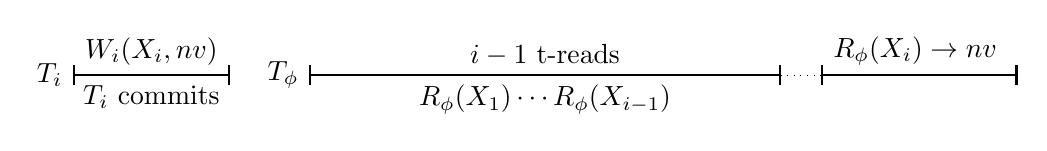
\begin{tikzpicture}
\node (r1) at (3,0) [] {};
\node (r2) at (7.7,0) [] {};

\node (w1) at (-2,0) [] {};


\draw (r1) node [below] {\normalsize {$R_{\phi}(X_1) \cdots R_{\phi}(X_{i-1})$}};
\draw (r1) node [above] {\normalsize {$i-1$ t-reads}};

\draw (r2) node [above] {\normalsize {$R_{\phi}(X_i)\rightarrow nv$}};

\draw (w1) node [above] {\normalsize {$W_i(X_i,nv)$}}; 
\draw (w1) node [below] {\normalsize {$T_i$ commits}};


\begin{scope}   
\draw [|-|,thick] (0,0) node[left] {$T_{\phi}$} to (6,0);
\draw [|-|,thick] (6.5,0) node[left] {} to (9,0);
\draw [-,dotted] (0,0) node[left] {} to (9,0);
\end{scope}
%
%
\begin{scope}   
%\draw [|-|,thick] (0,0) node[left] {$T_k$} to (6,0);
\draw [|-|,thick] (-3,0) node[left] {$T_i$} to (-1,0);
\end{scope}
%
\end{tikzpicture}
}}
        \\
        \vspace{2mm}
	\subfloat[fig2 \label{sfig:inv-2}]{\scalebox{0.6}[0.6]{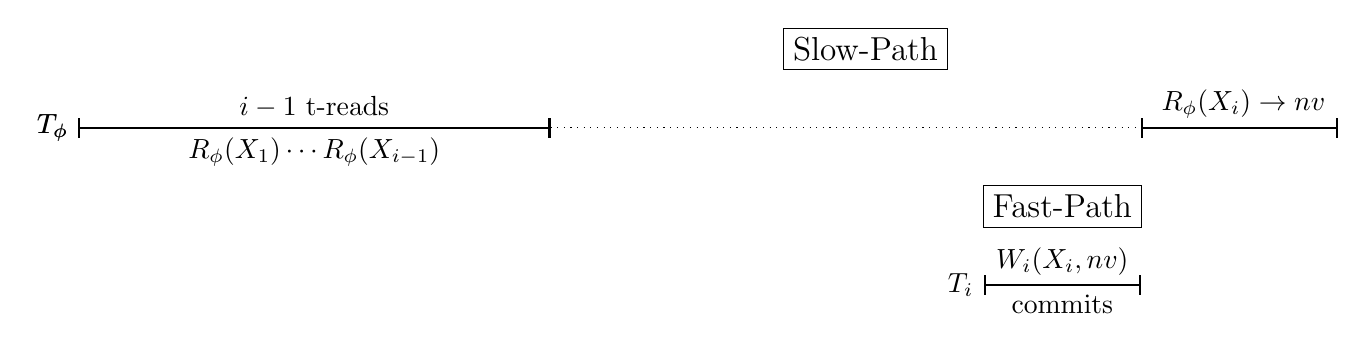
\begin{tikzpicture}
\node (r1) at (3,0) [] {};
%\node (r2) at (7.7,0) [] {};
\node (r3) at (14.8,0) [] {};

%\node (w1) at (7.5,-2) [] {};

\node (w2) at (12.5,-2) [] {};

\draw (r1) node [below] {\normalsize {$R_{\phi}(X_1) \cdots R_{\phi}(X_{i-1})$}};
\draw (r1) node [above] {\normalsize {$i-1$ t-reads}};

\draw (w2) node [above] {\normalsize {$W_{i}(X_{i},nv)$}}; 
\draw (w2) node [below] {\normalsize {commits}};

\draw (r3) node [above] {\normalsize {$R_{\phi}(X_{i})\rightarrow nv$}};
\node[draw,align=left] at (10,1) {{\large Slow-Path}};
\node[draw,align=left] at (12.5,-1) {{\large Fast-Path}};


\begin{scope}   
\draw [|-|,thick] (0,0) node[left] {$T_{\phi}$} to (6,0);
\draw [|-|,dotted] (0,0) node[left] {$T_{\phi}$} to (16,0);
\draw [|-|,thick] (13.5,0) node[left] {} to (16,0);
\end{scope}
%
%
\begin{scope}   
%\draw [|-|,thick] (0,0) node[left] {$T_k$} to (6,0);
\draw [|-|,thick] (11.5,-2) node[left] {$T_i$} to (13.5,-2);
\end{scope}
%
\end{tikzpicture}
%}}
	\caption{proof steps~\ref{sfig:inv-1}
        \label{fig:indis}} 
\end{center}
\end{figure*}
%
%%%%%%%%%%%%%%%%%%%%%%%%%%%%%%%%%%%%%%%%%%%%%%%%
\subsection{Progressive HyTM}
\label{sec:hytm2}
%
We can now prove the following theorem:
%
\begin{theorem}
\label{th:inswrite2}
There exists an opaque HyTM implementation that provides invisible reads
such that (1) in every execution $E$,
every fast-path transaction $T\in \ms{txns}(E)$
accesses one metadata base object,
(2) every execution $E$ is fast-path progressive or for
every fast-path transaction $T\in \ms{txns}(E)$
that returns $A_k$ in $E$, there exists an updating slow-path transaction $T_m \in \ms{txns}(E)$
concurrent to $T_k$.
\end{theorem}
%
\begin{proofsketch}
% 
\end{proofsketch}
%%%%%%%%%%%%%%%%%%%%%%%%%%%%%%%%%%%%%%%%%%%%%%%
%
\begin{algorithm*}[!ht]
\caption{Opaque HyTM implementation with sequential slow-path and progressive fast-path TM-progress; code for $T_k$ by process $p_i$}
\label{alg:inswrite2}
\begin{algorithmic}[1]
  	\begin{multicols}{2}
  	{
  	\footnotesize
	\Part{Shared objects}{
		\State $v_j \in \mathbb{D}$, for each t-object $X_j$ 
		%\Statex ~~~~~allows reads, writes
		\State $r_{j}$, sequence lock for each t-object $X_j$
		\State $L$, global single-bit lock
		%\Statex ~~~~~allows reads, writes 
		%\State implemented from reads and writes
		%\State $L$, multi-trylock
	}\EndPart	
% 	\Statex
% 	\Part{Process local objects}{
% 		\State $\Rset(T_k)$, storing $\{X_j,r_j\}$
% 		\State $\Wset(T_k)$, storing $\{X_j, v_j\}$
% 	}\EndPart
	\Statex
	\textbf{Code for fast-path transactions}	
	\Statex
	\Part{$\textit{start}_k()$}{
		
		\State $l \gets \Read(\ms{L})$ \Comment{cached read} 
		\If{$\ms{l} \mathrel{\&} 1\neq 0$}
			    \Return $A_k$ \EndReturn
		\EndIf
		
	}\EndPart
	\Statex
	%\Comment{In general, would it better to buffer writes in tryC?}
	\Part{$\textit{read}_k(X_j)$}{\quad\Comment{fast-path}
		
		\State $\textit{ov}_j := v_j.\Read()$ \Comment{cached read} 
		
		\Return $\textit{ov}_j$ \EndReturn
		
   	 }\EndPart
	\Statex
	\Part{$\textit{write}_k(X_j,v)$}{\quad\Comment{fast-path}
	
	\State $\underline{\textit{or}_j := \Read(r_j)}$ \Comment{uncached read}
	\State $\underline{r_j.\Write({or}_j+2)}$ \Comment{uncached write}
	\State $v_j.\Write(v)$ \Comment{cached write}
	\Return $\ok$ \EndReturn
		
   	}\EndPart
	\Statex
	
	%\Statex	
	\Part{$\textit{tryC}_k$()}{\quad\Comment{fast-path}
		%\Return $C_k$ \EndReturn
		\State $\ms{commit-cache}_i$ \Comment{returns $C_k$}
		
   		
   	 }\EndPart		
   	 \Statex
	\Statex
	\textbf{Code for slow-path transactions}
	\Statex
	\Part{$\textit{start}_k()$}{
		
		\State $l \gets \Read(\ms{L})$
				
	}\EndPart
	\Statex
	\Part{\Read$_k(X_j)$}\quad\Comment{slow-path}{
		  \If{$X_j\in \Wset(T_k)$}
		    \Return $\Wset(T_k).\lit{locate}(X_j)$ \EndReturn
		  \Else
		  \State $\textit{ov}_j := \Read(v_j)$ 
		  \State $\textit{or}_j := \Read(r_j)$ 
		  \State $\Rset(T_k) := \Rset(T_k)\cup\{X_j,or_j\}$ 
		  \If{$\textit{or}_j$ $\mathrel{\&} 1$}  	
			\Return $A_k$ \EndReturn
		  \EndIf
		  \If{$\neg \lit{validate}()$}
			\Return $A_k$ \EndReturn
		  \EndIf
		  \EndIf
		  \Return $\textit{ov}_j$ \EndReturn
		
   	 }\EndPart
   	\newpage
	\Part{\Write$_k(X_j,v)$}\quad\Comment{slow-path}{
		
			\State $\textit{nv}_j := v$
			\State $\Wset(T_k) := \Wset(T_k)\cup\{X_j,nv_j\}$
			\Return $\ok$ \EndReturn
		
   	}\EndPart
	\Statex
	
	%\Statex	
	\Part{\TryC$_k$()}\quad\Comment{slow-path}{
		\If{$\Wset(T_k)= \emptyset$}
			\Return $C_k$ \EndReturn 
		\EndIf
				
		\While {$\neg flag$}
		  \State $flag \gets L.\lit{cas}(0,1)$
		\EndWhile
		\ForAll{$X_j \in Q$}	
			\State $or_j\gets r_j.\lit{read}()$ 
			 		
		\EndFor
		\Comment{First read, then write all: single barrier}
		\ForAll{$X_j \in Q$}	
			\State $r_j.\lit{write}(or_j + 1)$ 
			 		
		\EndFor
		\If{$\lit{validate}()$}
			\State \textbf{goto} Line~\ref{line:release}
			
		\EndIf
		
		\ForAll{$X_j \in \Wset(T_k)$}
	 		 \State  $v_j.\lit{write}(\textit{nv}_j)$
			 
			 
	 	\EndFor		
		
  		\ForAll{$X_j \in \Wset(T_k)$}	\label{line:release}
 			\State $r_j.\lit{write}(or_j + 1)$ 
		\EndFor
		
		\State $L.\lit{write}(1)$
   		\Return $C_k$ \EndReturn
   	 }\EndPart		
	\Statex
	\Part{Function: $\lit{validate}()$}{
		
		\If{$\exists X_j \in Rset(T_k)$:$(\textit{or}_j\neq \Read(r_j))$}
			\Return $\false$ \EndReturn
		  \EndIf
		
		 \Return $\true$ \EndReturn
	}\EndPart
	
% 	
	}
	\end{multicols}
  \end{algorithmic}
\end{algorithm*}

%%%%%%%%%%%%%%%%%%%%%%%%%%%%